\documentclass[conference,a4paper]{IEEEtran}
\usepackage{lipsum}
\usepackage{graphicx}
\usepackage{float}
\usepackage{cite}
\usepackage{array}

\begin{document}
\title{Semi-Automated Unmanned Ground Vehicle With Raspberry Pi and Arduino Uno }

\makeatletter
\newcommand{\linebreakand}{%
  \end{@IEEEauthorhalign}
  \hfill\mbox{}\par
  \mbox{}\hfill\begin{@IEEEauthorhalign}
}
\makeatother

\author{
  \IEEEauthorblockN{Dhruv Pathak}
  \IEEEauthorblockA{\textit{Computer Engineering} \\
    \textit{MPSTME, NMIMS University}\\
    Mumbai, India \\
    dhruv.pathak74@nmims.edu.in}
  \and
  \IEEEauthorblockN{Vrushit Patel}
  \IEEEauthorblockA{\textit{Computer Engineering} \\
    \textit{MPSTME, NMIMS University}\\
    Mumbai, India \\
    vrushit.patel60@nmims.edu.in}
  \and
  \IEEEauthorblockN{Shivansh Sharma}
  \IEEEauthorblockA{\textit{Computer Engineering} \\
    \textit{MPSTME, NMIMS University}\\
    Mumbai, India \\
    shivansh.sharma95@nmims.edu.in}
  \and
  \IEEEauthorblockN{Shrey Thapar}
  \IEEEauthorblockA{\textit{Computer Engineering} \\
    \textit{MPSTME, NMIMS University}\\
    Mumbai, India \\
    shrey.thapar19@nmims.edu.in}
}

\maketitle

\begin{abstract}
Remotely operated and monitored rovers will soon take over the IoT world due to their diverse set of applications in a variety of sectors. In our project, we aimed to create a rover which monitors and allows users to manage it remotely or travels in a semi-automated manner without human input by detecting objects in front of it using ultrasonic sensors. It also produces graphical feedback on the region it traverses (using a gyroscope), indicating the air quality, temperature, and humidity of its surroundings using several other sensors such as the air quality sensor and the temperature and humidity sensor. This gadget was built on the unique approach of utilising a serialised integration of Raspberry Pi and Arduino, along with Google Firebase as its cloud server database and an easy-to-use interface.
\end{abstract}

\begin{IEEEkeywords}
Internet of Things, Artificial Intelligence of Things, Unmanned Ground Vehicle, Ground Rover, Raspberry Pi, Arduino UNO.
\end{IEEEkeywords}

\section{Introduction}

Internet of Things (IoT) can be described as a network of devices consisting of sensors and computers using which one can collect, analyze, share and secure data.
It has been the trendsetter in new technological developments all over the world. The automobile industry has been shifting to autonomous vehicles and connected cars, IoT has played a massive role in this advancement\cite{8}. IoT devices give meaningful data on a variety of physical factors, allowing for increased productivity and resource utilisation while reducing human labour and, as a result, lowering errors. Governments at all levels can use IoT technologies to create smart solutions such as identifying the need for road maintenance by detecting the post holes based on the vibration of a device and monitoring the air quality index in various neighboring localities. Users benefit from enhanced road quality and safety because of IoT integration.

For implementing this project, we used a Raspberry Pi 3 B+ and Arduino UNO in a serialized manner wherein the Raspberry Pi is the brain of the system and Arduino is the body mainly used for controlling the movement of the system. Raspberry Pi has multiple advantages like providing support for multiple sensors and coding languages alongside having a fast processing speed enabling it to handle computationally expensive tasks like image processing. The Arduino UNO board includes a variety of hardware elements as well as the ability to communicate with a variety of modules such as the internet, Bluetooth, motor control, and other capabilities.

We also utilised a Pi camera to detect lanes and recognise obstacles. Ultrasonic and infrared sensors are employed for obstacle avoidance by calculating the distance between the vehicle and the object\cite{9}. Air quality sensor is used for identifying the quality of the air by displaying the composition of the gases around it in the air \cite{3}. Humidity and temperature sensors outputs the local temperature and humidity. For object detection, a cloud database has been set up for storing images dynamically. When the rover encounters an obstacle, the ultrasonic sensors measure the distance between the obstacle and the rover accordingly chart out the way forward for the rover.
There are various publications based on unmanned ground vehicles which employ either web-based controls or operate completely autonomously. The system which has been built here uses a GUI web based controller and has an autonomous mode.

\section{Related Work}
\subsection{Architecture}
Two micro-controller platforms were chosen to implement the system requirements: Raspberry Pi and Arduino \cite{11}.

The main tasks of Raspberry Pi are:
\begin{enumerate}
  \item Check for the internet connection
  \item It receives data from an Android application and sends it to an Arduino to drive the Unmanned Ground Vehicle (UGV).
  \item Live-streaming in  manual mode and video recording  in  autonomous mode.
\end{enumerate}

The main tasks of Arduino are: 
\begin{enumerate}
    \item It receives command data from the Raspberry Pi and performs actions such as controlling the direction of the mobile robot and controlling the direction of the camera  in manual mode.
    \item Check the  charge capacity of the battery.
    \item Save the starting point coordinates.
    \item Mathematical calculation between two coordinate points.
    \item Implement obstacle avoidance in the autonomous mode 
\end{enumerate}

\begin{figure*}[ht]
\centering
\includegraphics[width=1\linewidth]{IoT3a.png}
\caption{Architectural Layout of the system}
\label{Fig: IoT5}
\end{figure*}

\subsection{Cloud}
A third-party application provides cloud services for the project. Through the cloud, the Raspberry Pi connects with the Arduino and the third party application. It transfers the captured video to the server and subsequently delivers the user's input signal to the Arduino. An android application is designed to transfer live stream command signal with the system over the cloud. \cite{7}

\begin{figure}[ht]
\centering
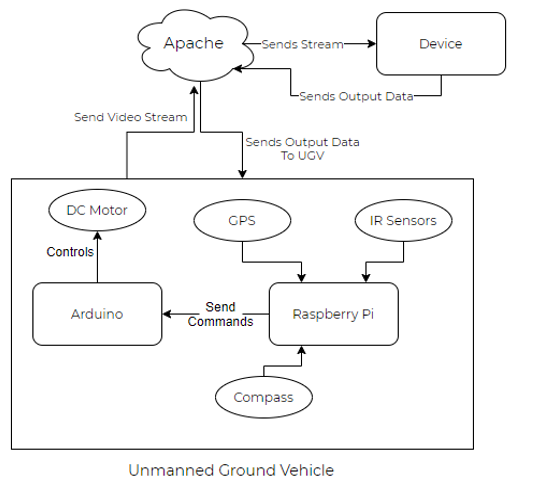
\includegraphics[width=1\linewidth]{IoT.jpg}
\caption{Cloud}
\label{Fig: IoT2}
\end{figure}

\subsection{Connectivity}
Pull-based communication is often used in Named Data Networking (NDN) to enable robust and sustainable message dissemination across the channel. It is a computational emerging IoT design that gets data on specified content and provides better results over TCP (Transmission Control Protocol) networking, such as content distribution efficiency and cyber security. NDN architecture differs from TCP/IP at the middle or ‘thin waist’ layer. The NDN model, instead of pushing data to IP locations, does a demand-pull of data. \cite{1}

\begin{figure}[ht]
\centering
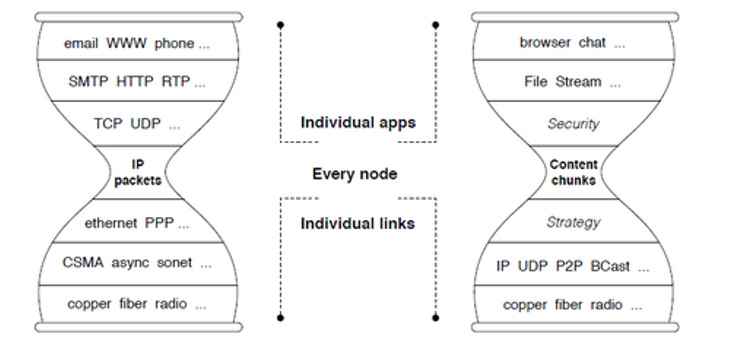
\includegraphics[width=1\linewidth]{IoT2.jpg}
\caption{Connectivity}
\label{Fig: IoT3}
\end{figure}

Security is incorporated into the data itself in NDN, rather than being determined by where or how it is received. Each piece of data is signed with its own unique name, securing the connection. Applications cannot "opt out" of security since data signatures are required.\cite{11}

\subsection{Controlling}
\subsubsection{Command Controlled Mode}
They have taken into account human decision-making in this mode, and deliver navigation orders based on the live visual feed received from the camera installed on the UGV.\cite{9}

\subsubsection{Self Controlled Mode}
Self-decision and navigation are based on vision, artificial intelligence, path planning, and obstacle detection algorithms in this mode. \cite{9}

\subsection{Gesture Controlled Mode}
Hand gesture signals are taken into account in this mode, and the UGV is controlled by instructions supplied based on the Inertial Measurement Unit (IMU) unit's mapping of hand motions \cite{9}.

\subsection{Raptor Controlled Mode}
In this mode, the motion tracking system has been considered implemented through advanced image processing algorithms to locate and eliminate targets in the field vision.

A study on road monitoring systems covers the following points\cite{2}:

Current road monitoring systems utilise smartphone applications for collecting data. The program requests permission from the user to utilise several detectors such as a gyroscope, an accelerometer and a GPS sensor. The smartphone is usually installed inside the vehicle using a mounting bracket during information gathering. After data collection, the application then sends the data back to the cloud database. For accurate recognition of road quality, the data from vibration sensors and other sources are processed using the DeepSense framework.

A study on air quality monitoring system which uses IoT covered\cite{3}:

Nodes constituted of a micro-controller, pollution sensors, and an RFID reader are strategically positioned along highways in this system. When a car equipped with RFID passes by the member nodes, it is recognised. As a result, the node measures the air quality created by the vehicle and communicates the data to the central server responsible for data storage.

\section{Proposed Model}

\begin{figure*}[ht]
\centering
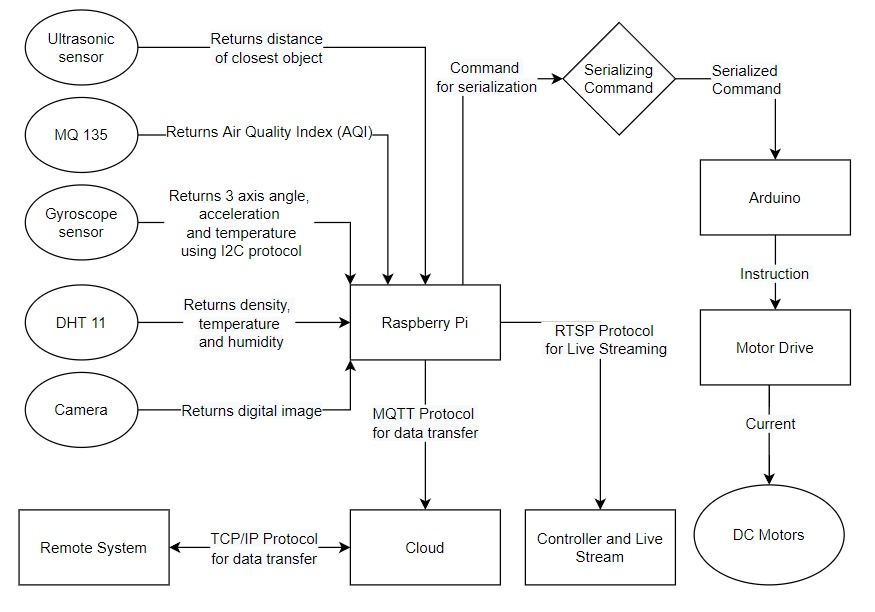
\includegraphics[width=1\linewidth]{architecture.jpeg}
\caption{Unmanned Rover Architecture}
\label{Fig: Arch}
\end{figure*}

\subsection{Hardware}
The major hardware components used to implement the given prototype are the Raspberry Pi and Arduino. The Raspberry Pi feeds the live stream to the server along with the sensor readings, while the Arduino is used for gaining control over the motor driver circuit. Serial connection is needed to link the Raspberry Pi to the Arduino so that the Arduino can be instructed on how to drive the vehicle.
\subsubsection{Arduino}
The Arduino UNO is a low-cost, adaptable, and simple accessible configurable micro-controller board that may be used in a wide range of applications. As an output, this board can control switches, Led displays, servo motors, and wheels and can be wired up with several other Arduino boards, shields, and Raspberry Pi boards.

\begin{figure}[ht]
\centering
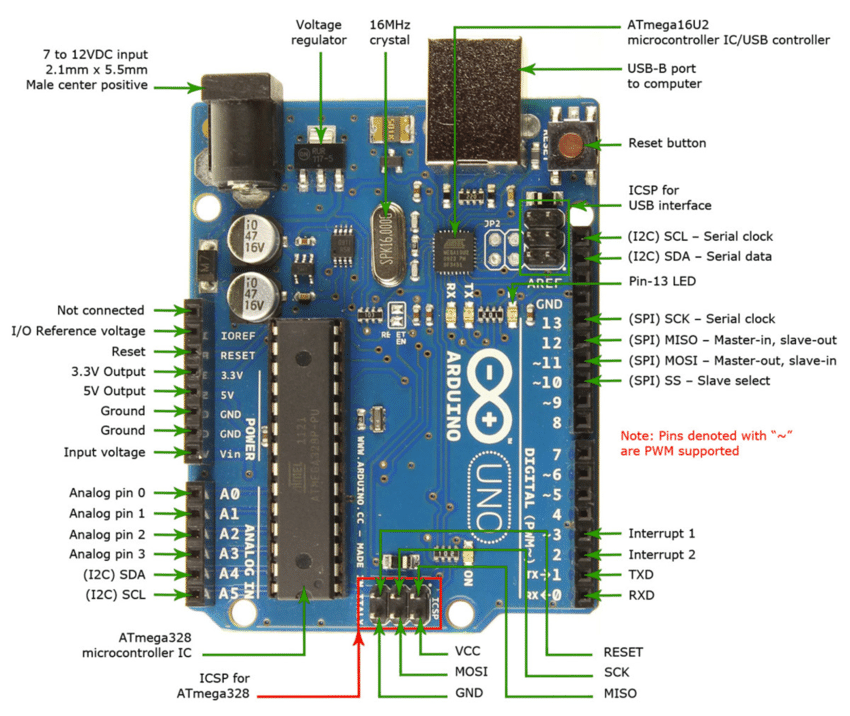
\includegraphics[width=1\linewidth]{ArduinoUNO.jpg}
\caption{Arduino UNO Model}
\label{Fig: Model}
\end{figure}

Arduino UNO micro-controller boards are capable of reading inputs - lights on a sensor or a LED, activates and operates a motor \cite{5}. It comprises of 14 digital I/O pins, 6 analogue inputs, a reset button, a power jack and a USB connection. 
Arduino is an open source electrical platform that sends a set of instructions to the Arduino micro-controller and is built on a user friendly hardware and software. To do this, With Arduino software (IDE), Arduino creates its own programming language based on processing \cite{10}. 
Connecting the Arduino to a computer through a USB cable or power it using an AC-to-DC converter or battery initiates the system\cite{10}. One can experiment about with the UNO without fear of anything going haywire with the worst-case scenario being the replacement of a cheap chip and starting again.

\subsubsection{Raspberry Pi}
The Raspberry Pi is a computer based on a single board which is the size of a bank card. There are now four Raspberry Pi versions on the market: the Model B+, Model A+, Model B, and Model A. Each of these versions use the same systems on chip, which combines a CPU and a GPU chip, with the only difference being the hardware and software features each of them have to offer \cite{4}.
In this project, we have used the B+ model. It has 40 GPIO pins, 4GB RAM and 64GB storage, apart from which it also supports wireless connections and has a Gigabit Ethernet port. Raspberry Pi can be employed in wide range of domain, such as for weather monitoring, security cameras etc. because of its low cost, modularity, and open design \cite{12}.

\begin{figure}[ht]
\centering
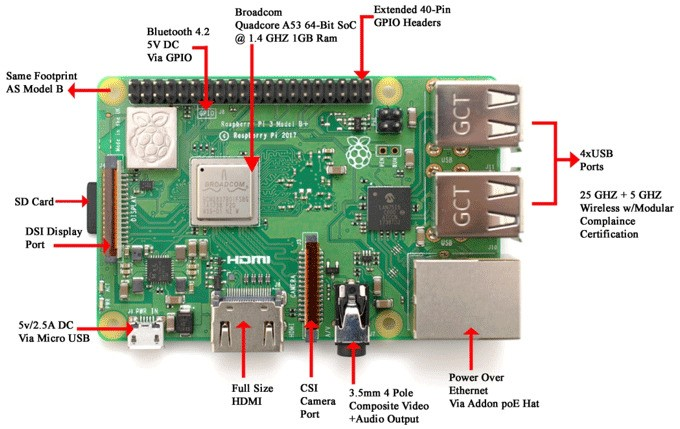
\includegraphics[width=1\linewidth]{RasPi.jpg}
\caption{Raspberry Pi 3B+ \cite{4}}
\label{Fig: Pi}
\end{figure}

\subsubsection{Body}
Polyactic Acid (PLA) has been used to 3-D print the rover's body. PLA is a thermoplastic polymer made from natural materials like maize starch or sugar cane \cite{20}. While PLA has several drawbacks over its competitors, such as lower heat resistance and tensile strength, it is compensated for by its simplicity of usage and post-processing. The body has been precisely produced, with spaces left in it for organising the wires in a logical manner.

\begin{figure}[ht]
\centering
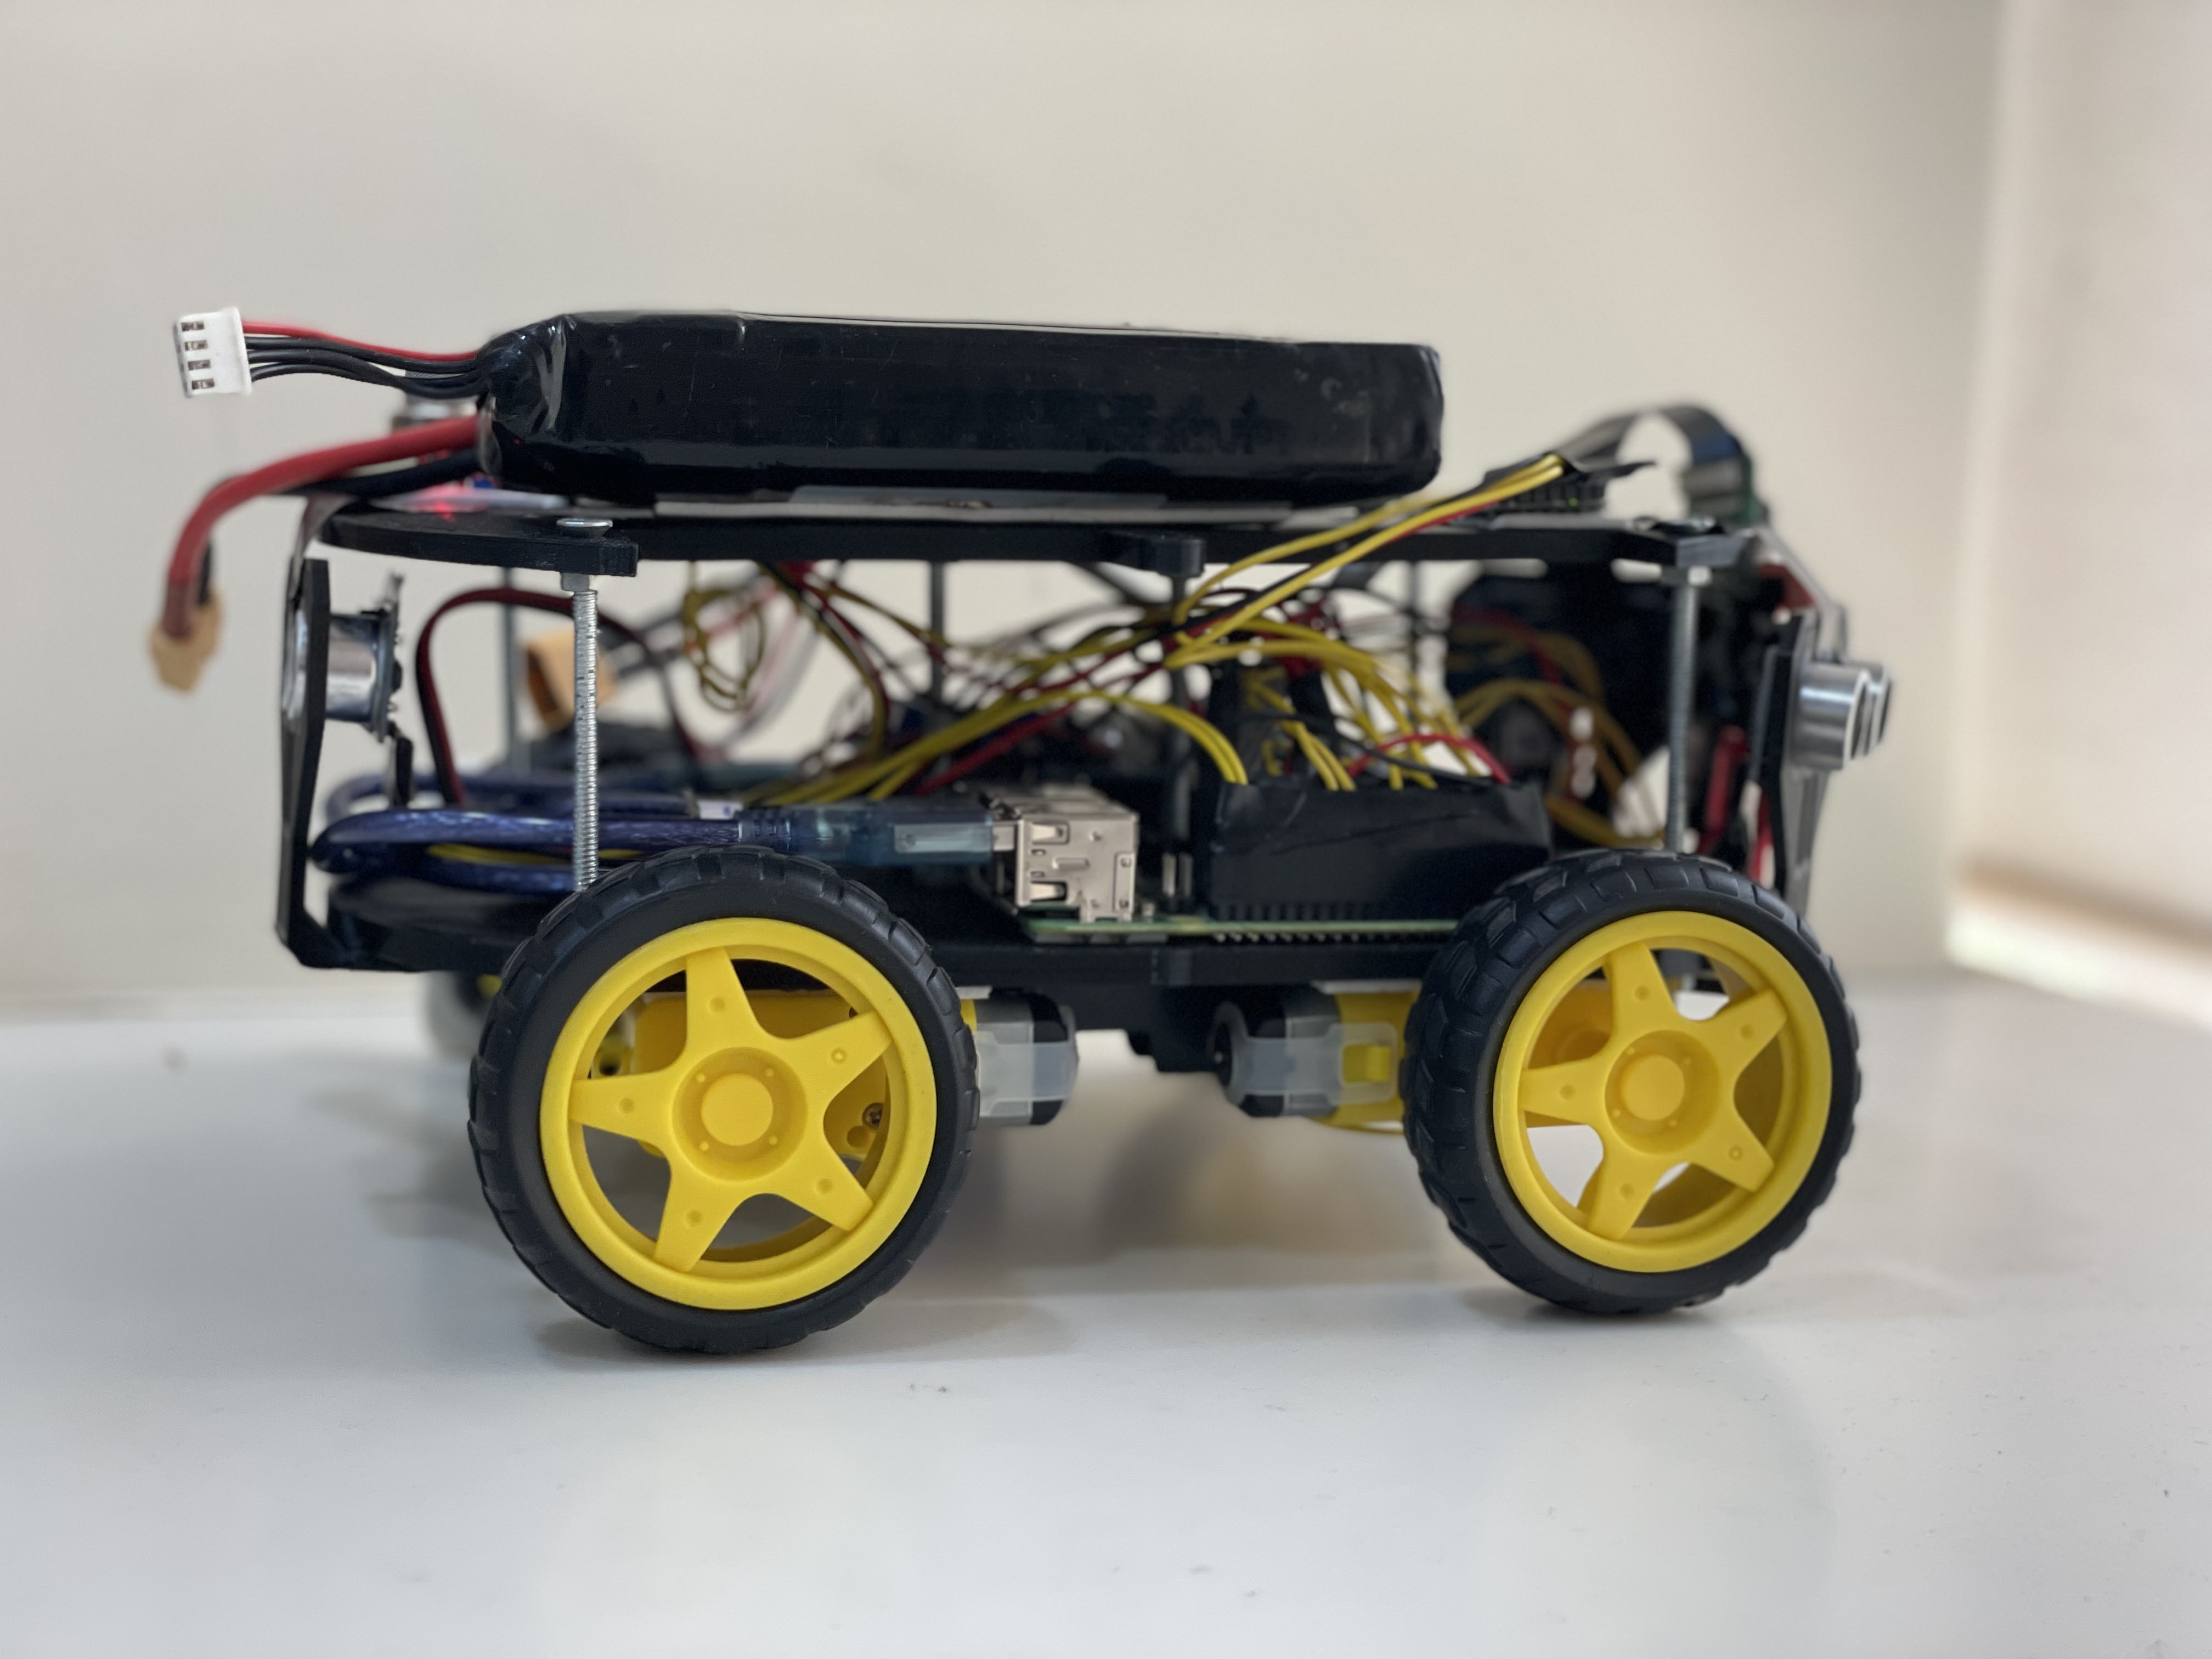
\includegraphics[width=1\linewidth]{Roverside.jpg}
\caption{Side view of Rover}
\label{Fig: Rover Side}
\end{figure}

\begin{figure}[ht]
\centering
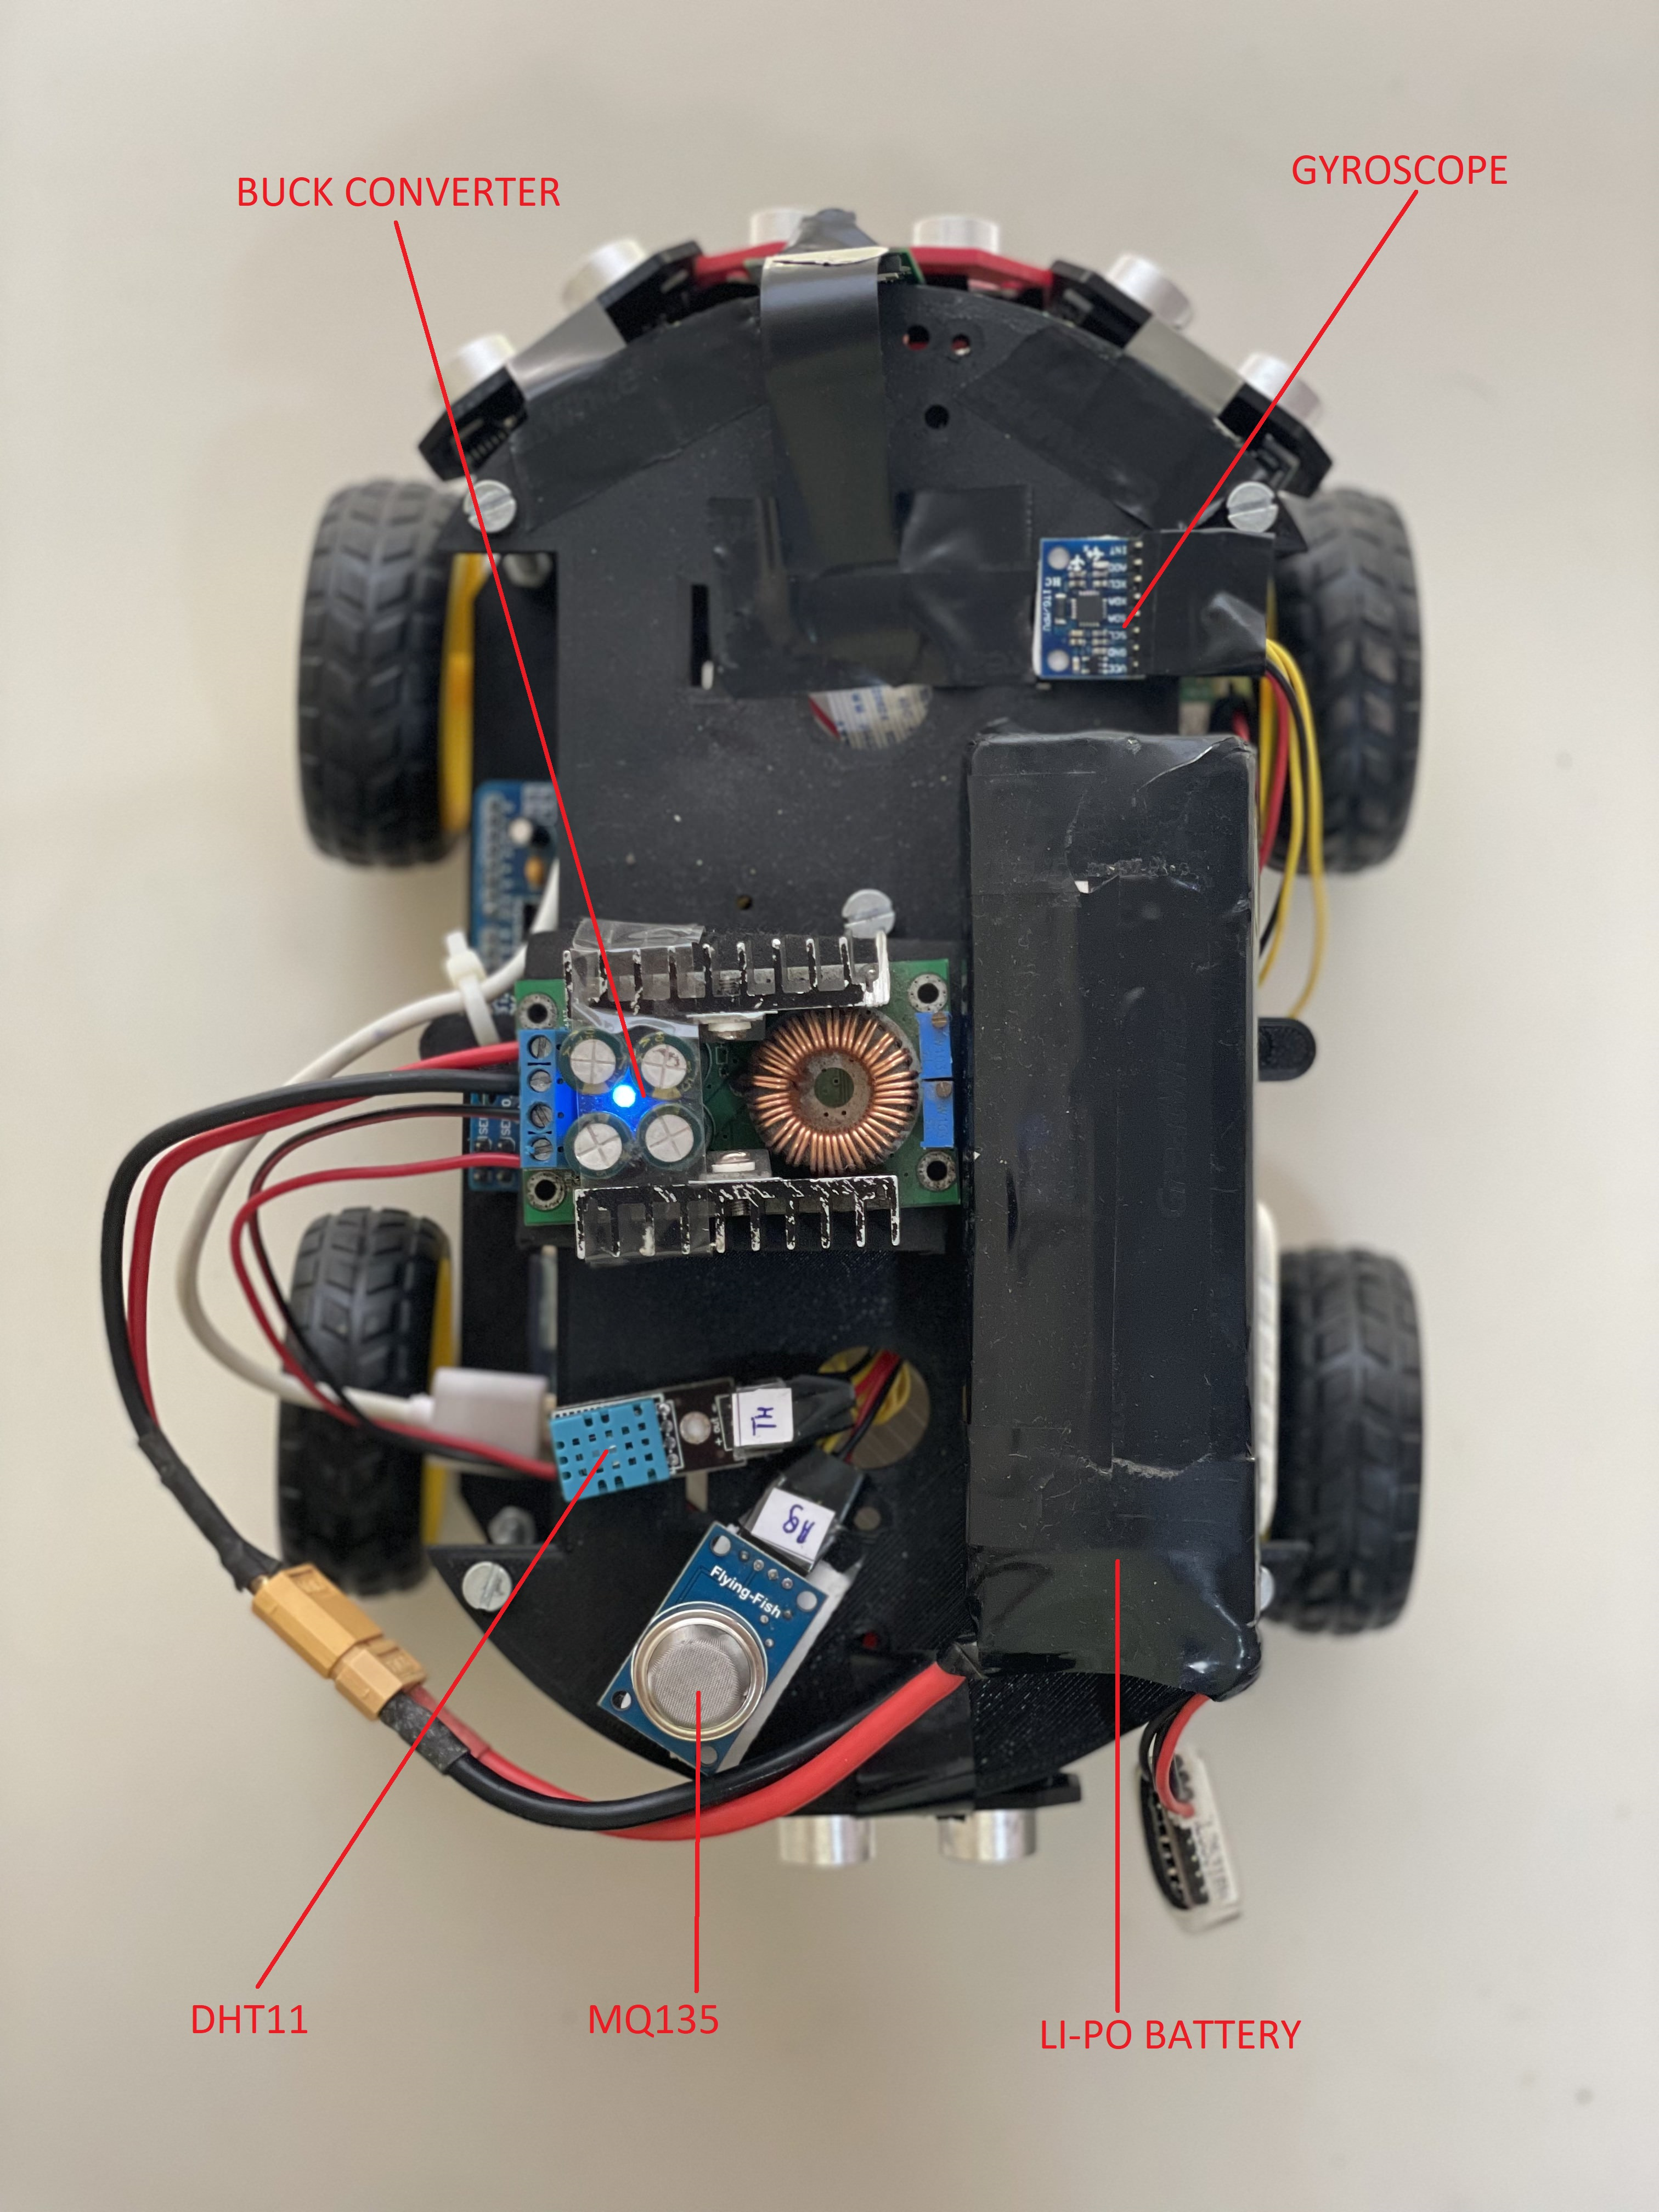
\includegraphics[width=1\linewidth]{Rovertop.jpg}
\caption{Top View of Rover}
\label{Fig: Rover Top}
\end{figure}

\begin{figure}[ht]
\centering
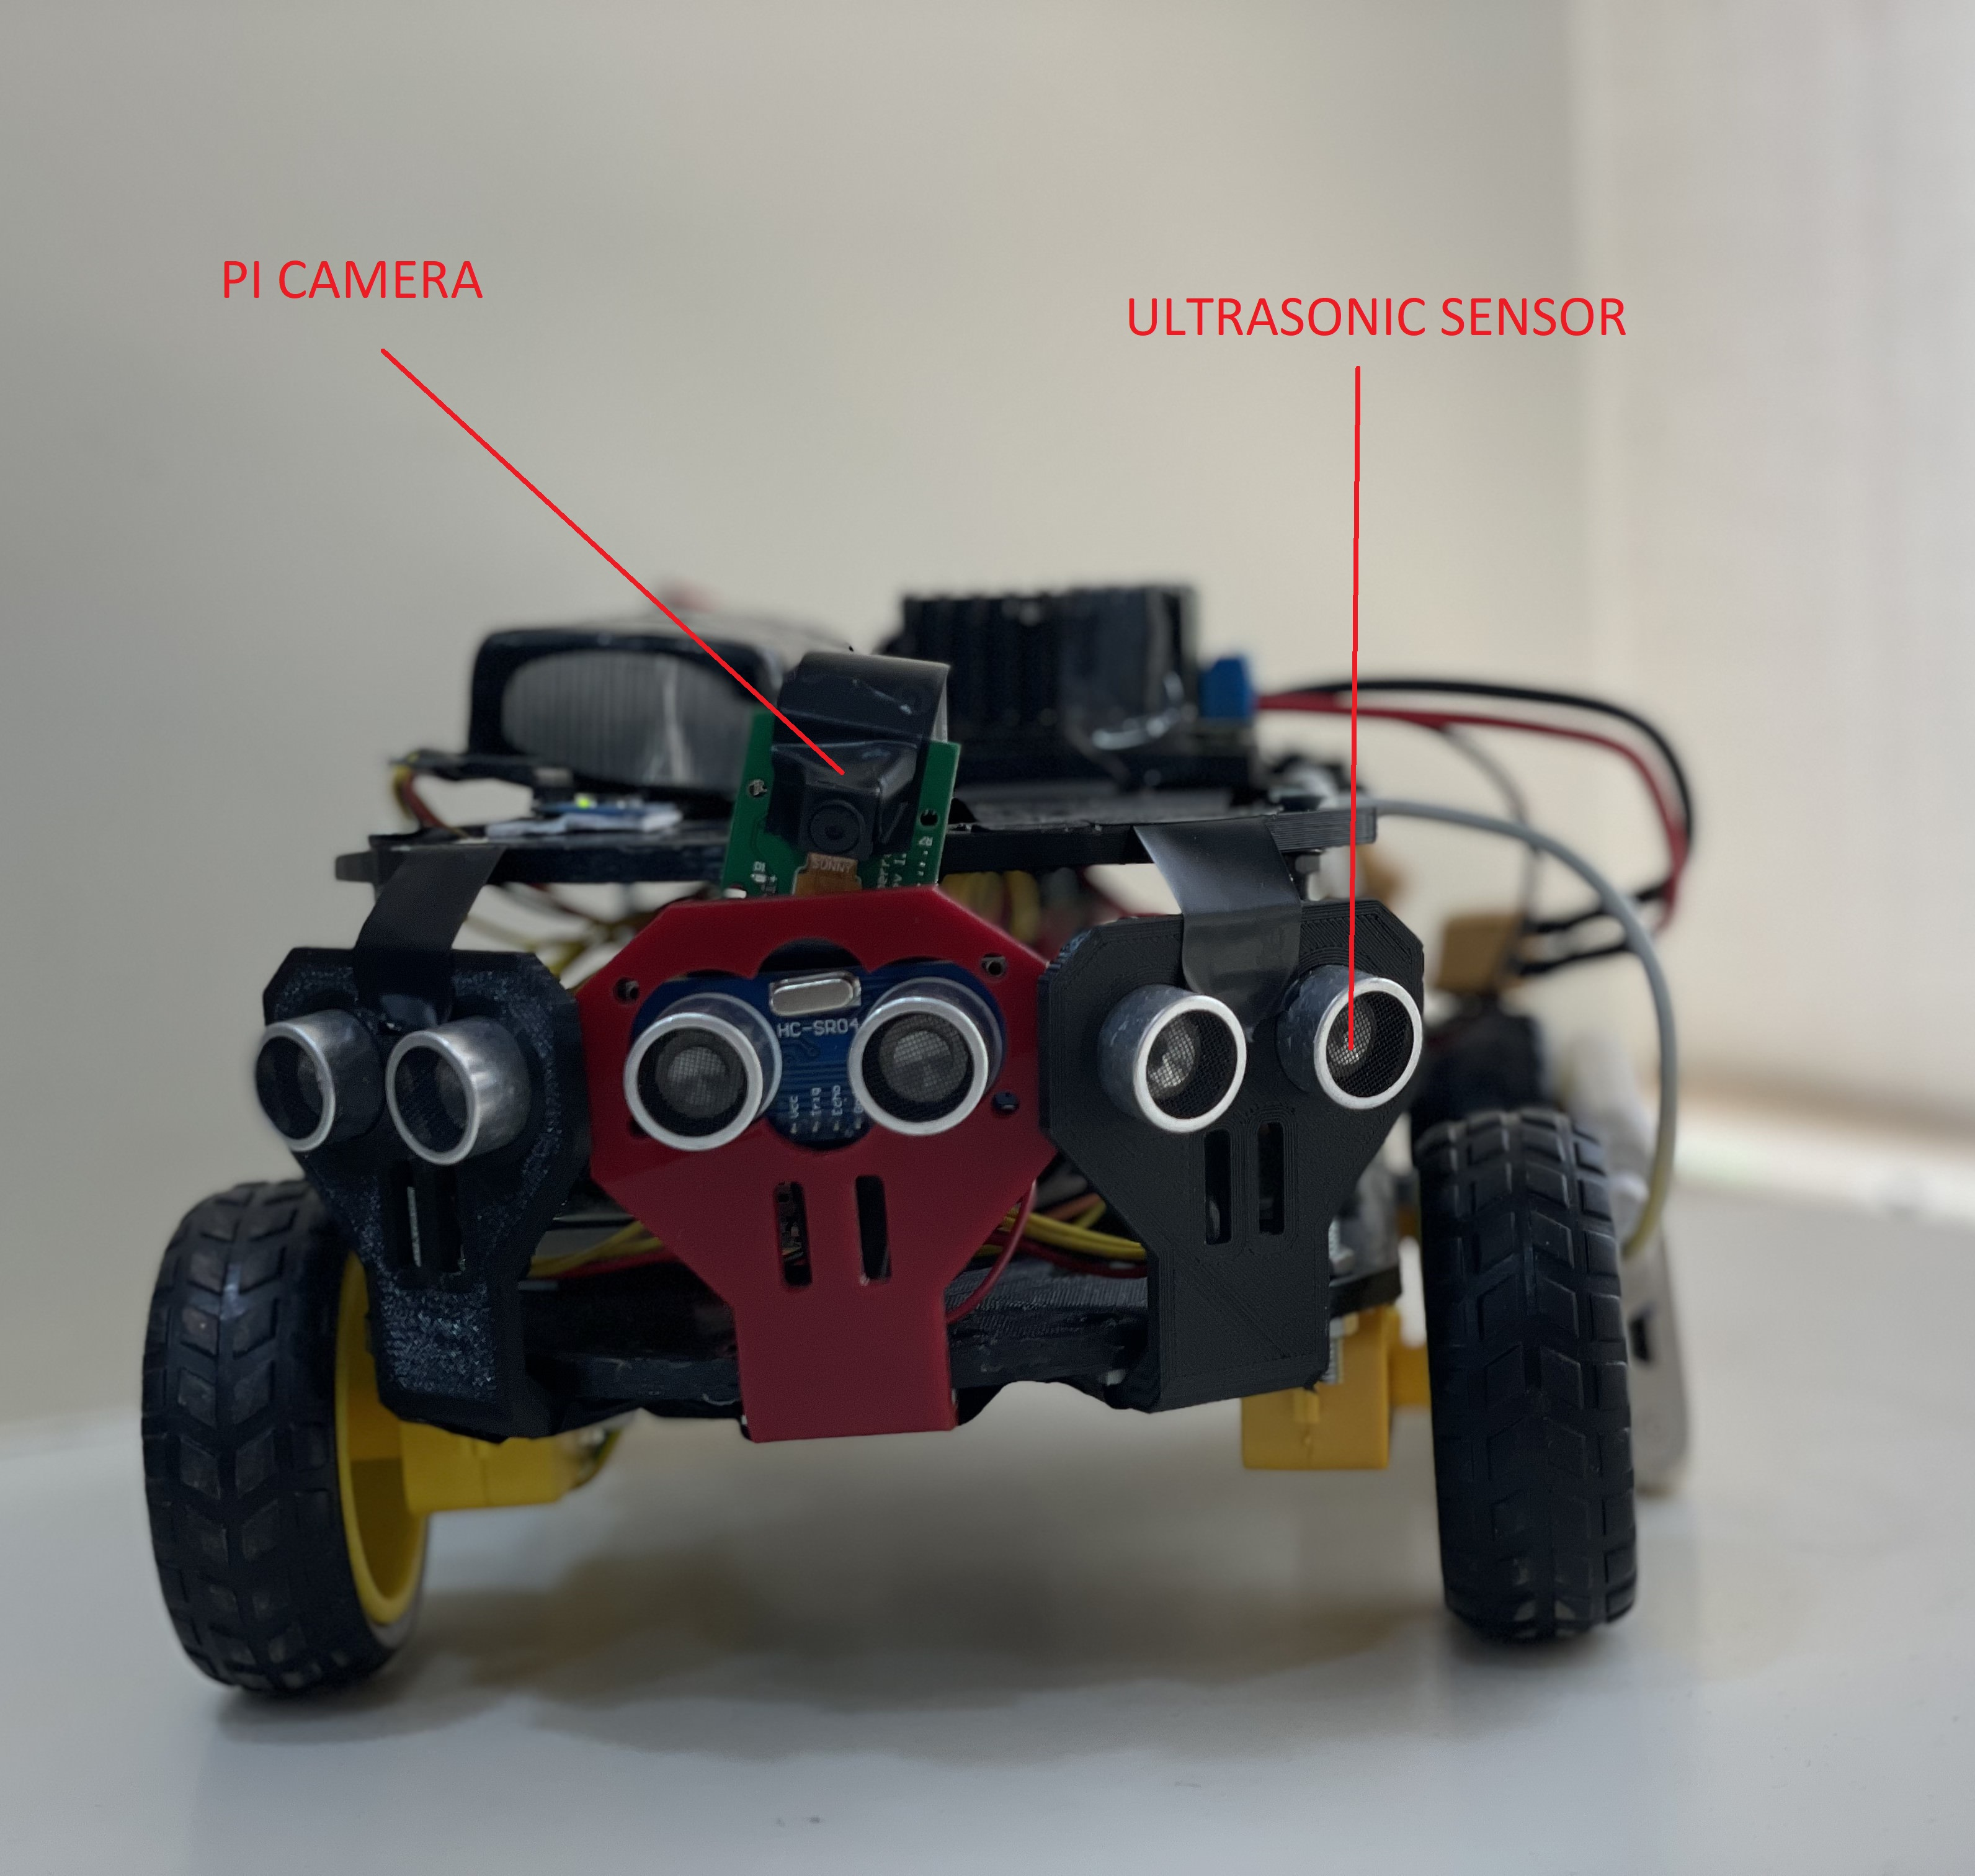
\includegraphics[width=1\linewidth]{Roverfront.jpg}
\caption{Front view of Rover}
\label{Fig: Rover Front}
\end{figure}

\subsubsection{Gyroscope}
A gyroscope is a Micro Electro-Mechanical Systems (MEMS) sensor which has the capability of mapping the co-ordinates of its location in the 3 axes - x-axis, y-axis and z-axis. This sensor continuously measures the acceleration of it's surroundings and reports it in the output.
The use of the gyroscope sensor in this project is for finding the quality of the road where the rover travels and report it successfully. \cite{13} The working of this sensor is really simple, for getting the quality of the road, a graph can be made with 2 axes, the x-axis and the z-axis. The x-axis would show that the vehicle was moving and the z-axis maps the elevation of the rover. If the z-axis reports a value below the average reported value of a trip, it would refer the road has been damaged and had potholes there.

\subsubsection{Camera}
The Raspberry Pi Camera Board is a plug-and-play module that connects to the Raspberry Pi through a ribbon connection. The sensor has a resolution of 5 megapixels and can capture films at 1080p at 30 frames per second and 720p at 60 frames per second.

\subsubsection{Ultrasonic Sensor}
Using ultrasonic sound waves, an ultrasonic sensor computes the distance between itself and an object. The Ultrasonic sensor is used here for automation in the movement of rover, using which the rover can move around and know before hand of the obstacles which come in its range of movement.\cite{14}

Ultrasonic sensors work by emitting sound waves at frequencies exceeding the range of the human ear. The detector has a component known as the sensor's transducer, which functions as a mic for delivering or receiving ultrasonic sound. The device calculates the distance between the object and itself by monitoring the duration between transmitting and receiving ultrasonic pulses.\cite{15}

\subsubsection{Air Quality Sensor}
Air quality sensors are inexpensive and portable devices used to detect pollutants in the air comprising of particles, contaminants, and noxious gases that are potentially hazardous to human health. The air quality sensors are linked to the Arduino UNO micro-controller, and the data collected by the sensors is saved in a cloud database and shown on the web application. \cite{16}

\subsubsection{Battery}
Lithium polymer (Li-Po) batteries are used to power the motor shields connected to the Arduino UNO board. Li-Po batteries are connected in series, and if you place regular batteries in series, the voltage of each cell will be different after use, and the charging time of each cell will be uneven, so you will get the desired voltage.

To solve this problem, you can use the Li-Po battery to charge each cell of the battery individually to prevent overcharging of the battery cell. Lithium-ion batteries provide features such as improved charge – discharge frequencies, longevity, high efficiency, and affordability, as well as a lightweight structure. \cite{19}

\subsubsection{Hobby Motor}
The Arduino Motor Shield allows the user to simply regulate the position and momentum of the motor using the Arduino. Support for Arduino pins is easy, so one can easily add motors to the project. One can also operate the motor with another power pack up to 12V.

\begin{figure}[ht]
\centering
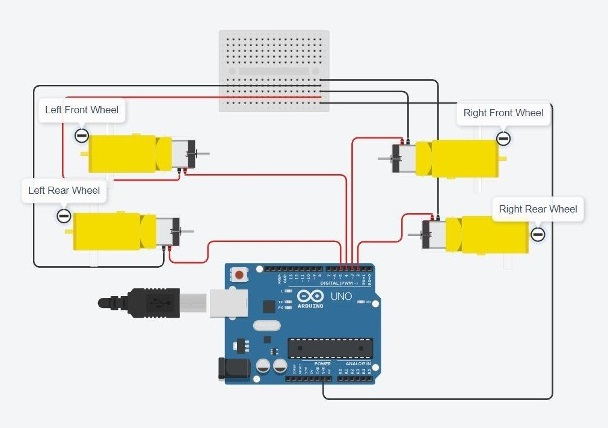
\includegraphics[width=1\linewidth]{Hobby.jpg}
\caption{Hobby Motor Wheel Setup}
\label{Fig: Hobby}
\end{figure}

The most common engine foam is a DC motor. Most DC motors have  two leads. Plus and negative. If these two lines are directly connected to the battery, the motor rotates. When the line is switched, the motor rotates in the other direction.  
Hobby motors are controlled as four driven drives for the robber. By controlling different combinations of  four motors, we have developed four basic movements: forward, backward, left and right.

\begin{figure}[ht]
\centering
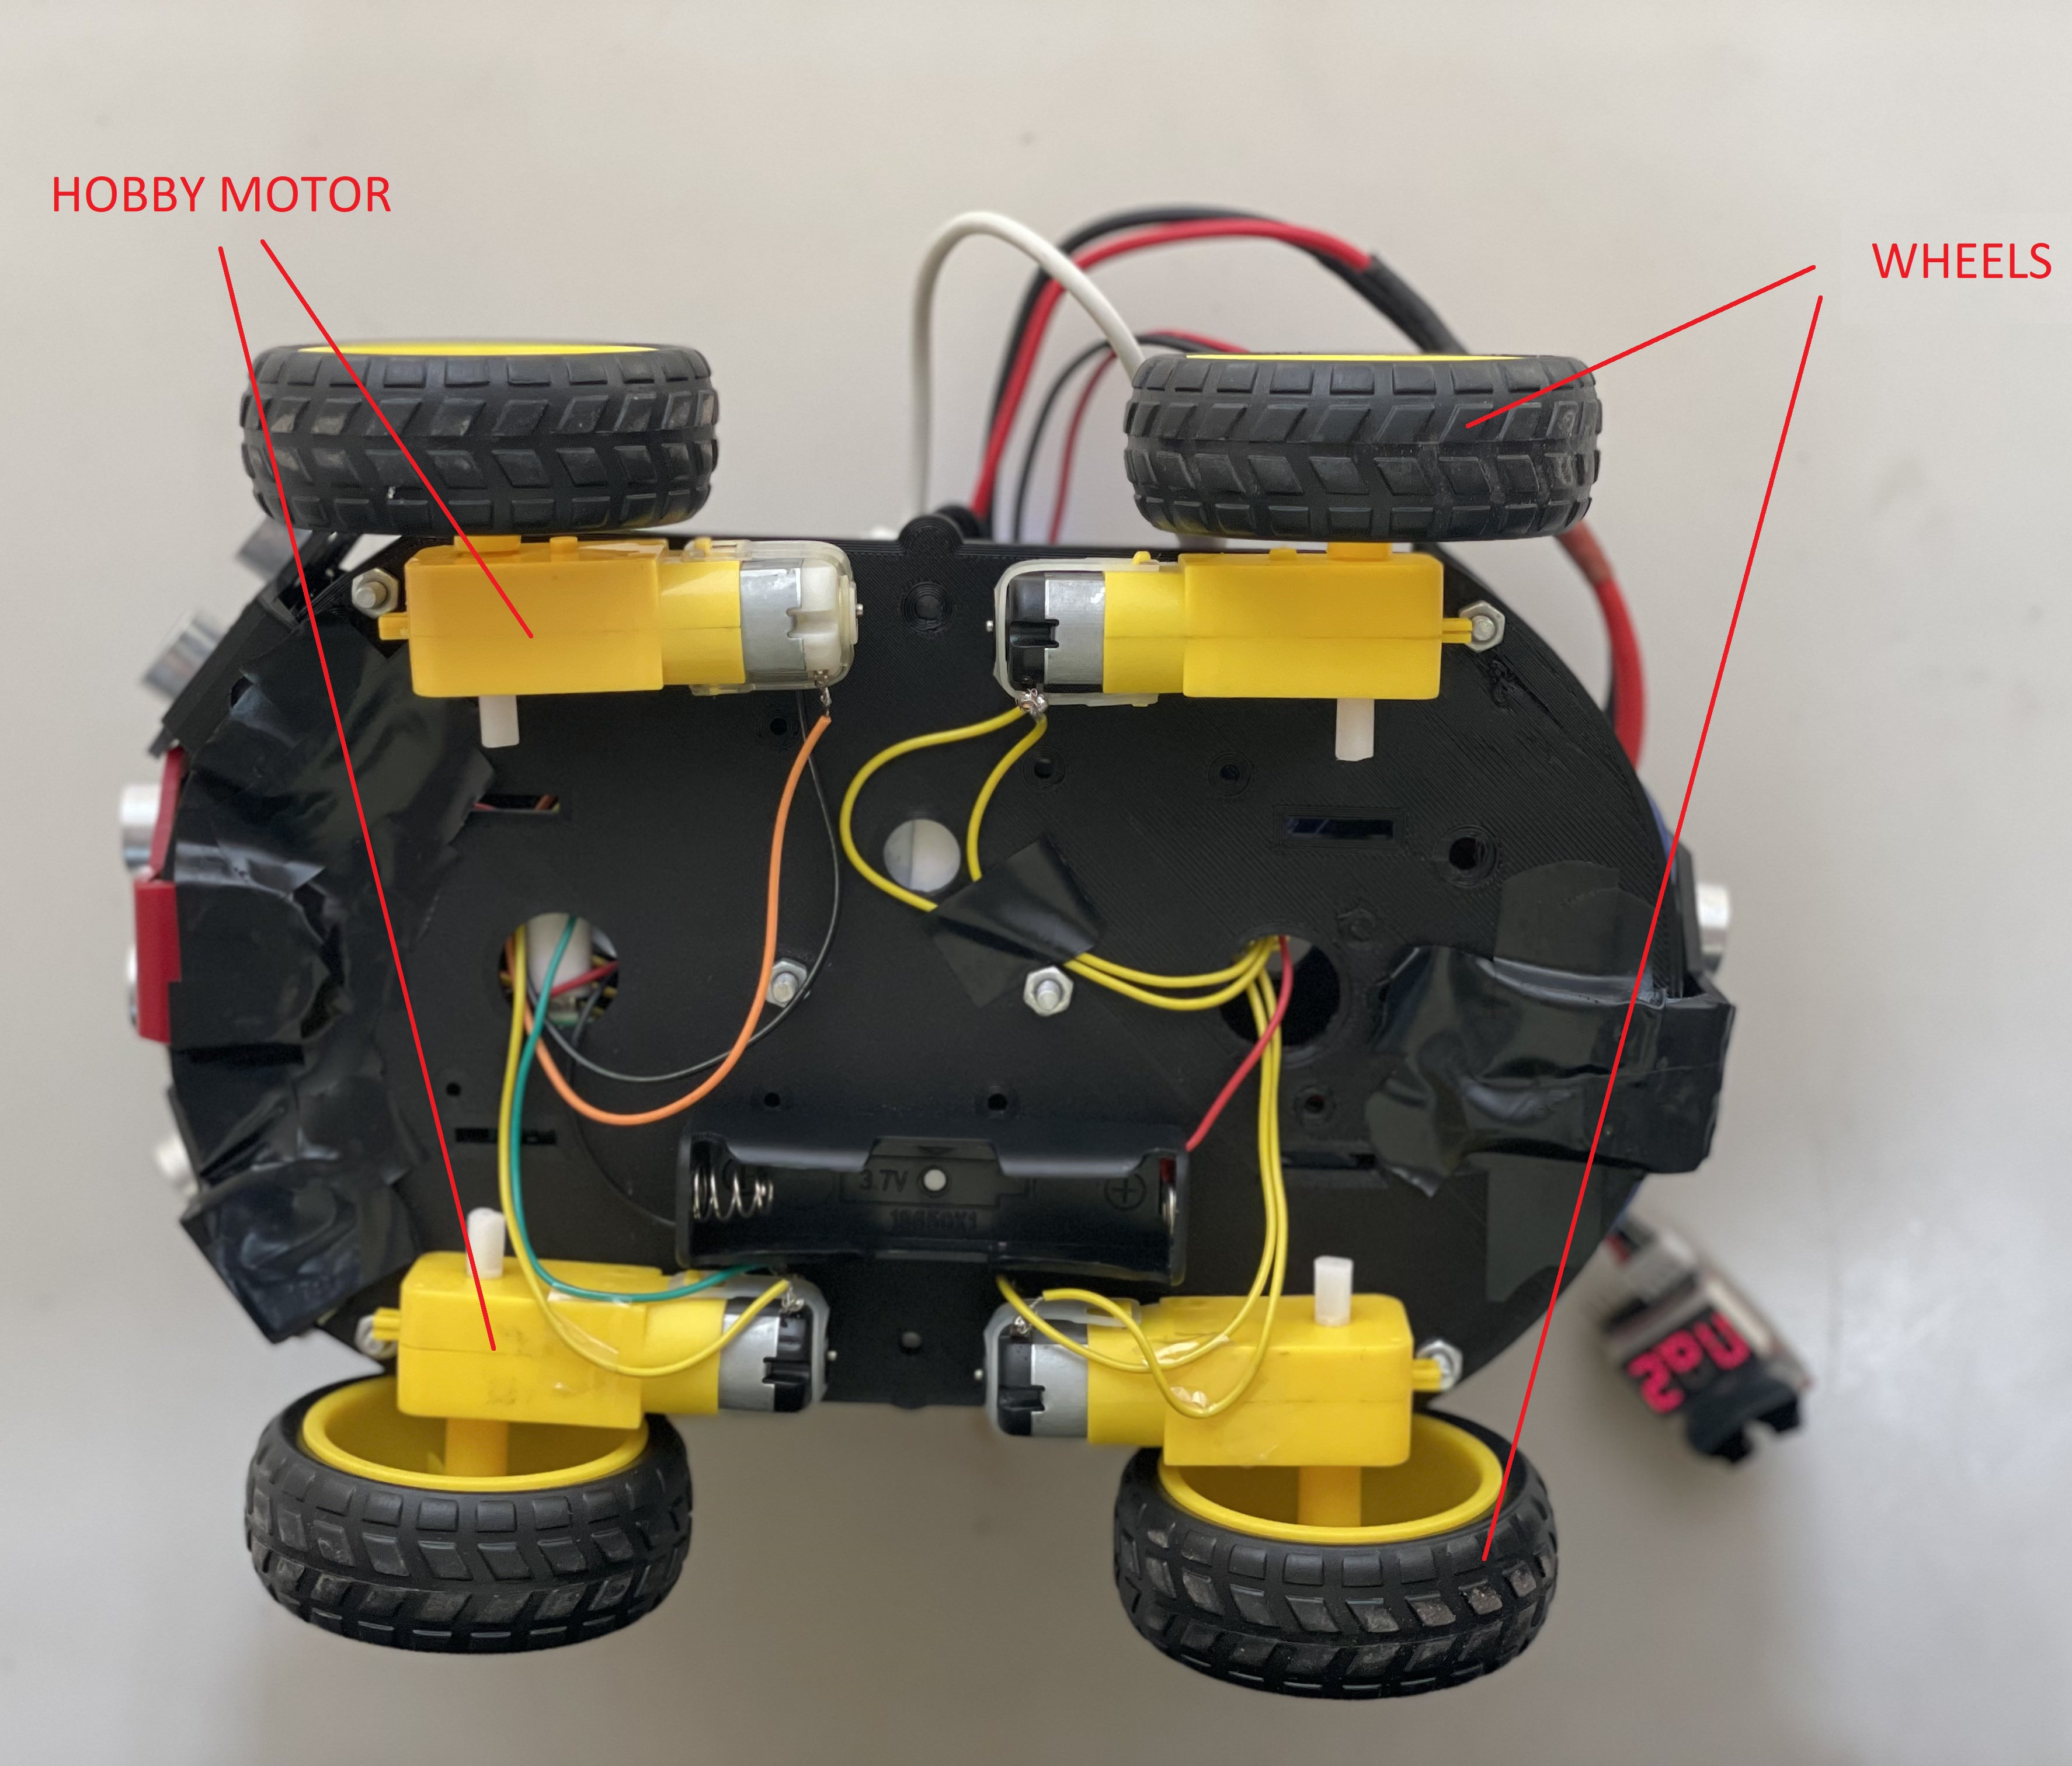
\includegraphics[width=1\linewidth]{Roverbottom.jpg}
\caption{Hobby Motor arrangement in Rover}
\label{Fig: Hobby Arrangement}
\end{figure}

Serial Commands for DC Motor: Serial communication is only a data communication link. The data will be sent every bit at a time and 1 byte = 8 bits. In contrast to parallel communication, which sends bits at the same time, serial communication transmits bits sequentially, which make is faster than serial communication.

\subsubsection{Buck Converter}
The Li-Po battery in the rover produces a really high amount of voltage than the required amount for powering the motors, thereby requiring a buck converter with a constant current, constant voltage (CC-CV) method. The buck converter then efficiently converts the high DC voltage generated by the Li-Po battery to a low DC voltage, extending battery life and lowering the heat output
\cite{18}.

\subsubsection{Density, Humidity and Temperature Sensor (DHT11)}
The DHT11 is a relatively cheap digital temperature and humidity sensor. Any micro-controller may simply communicate with this sensor.

\subsection{Major Software and Languages Used}
\subsubsection{Raspberry Pi OS}
The Raspberry Pi OS is a Linux-based operating system that powers the Raspberry Pi. All versions are distributed as .img disk image files. These files may then be loaded onto micro-SD cards, which are used to run the Raspberry Pi OS.

\subsubsection{Python}
Python is an interpreted programming language that enables the Raspberry Pi to communicate with a user or client in order to control the system's movement.

\subsubsection{Putty and SSH} 
Putty is a third party software that is used in the system for establishing SSH sessions between the Raspberry Pi 3 module and a Windows laptop with the goal to view and manage the module's command terminal on the machine. \cite{6} SSH (Secure Shell) is a software package that is used for generating various Shell sessions running on cryptographic networks protocols.

\subsubsection{Serialization}
Serialisation is the process through which Raspberry Pi and Arduino can communicate, it is a straightforward method of data transport. 

\begin{figure}[ht]
\centering
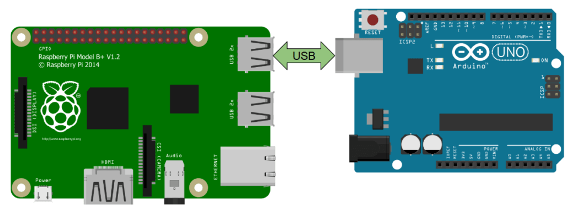
\includegraphics[width=1\linewidth]{serial.png}
\caption{Serialization Communication}
\label{Fig: Seralization}
\end{figure}

The data is transmitted progressively, one bit at a time. Both devices can commence communication in serialisation \cite{17}.

\subsubsection{Firebase Cloud Services}
Google Firebase is a Google-backed application development software that enables developers to store real-time data on the cloud. To send data from the Raspberry Pi to our Firebase cloud storage, we use the unique Firebase API key generated on the cloud and place it in the code.

\begin{figure}[ht]
\centering
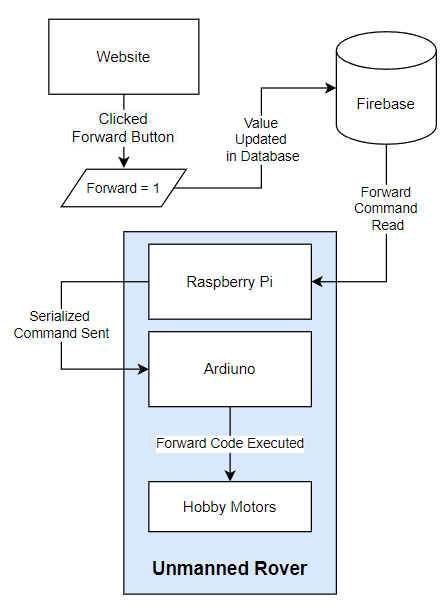
\includegraphics[width=1\linewidth]{controller.png}
\caption{Forward Control over the Internet}
\label{Fig: Control}
\end{figure}

\section{Implementation}

\subsection{Working}
The working of the unmanned rover has been divided into multiple sections:

\subsubsection{User Interface and Functionality}
The web application displays the following modules:
\begin{figure*}[ht]
\centering
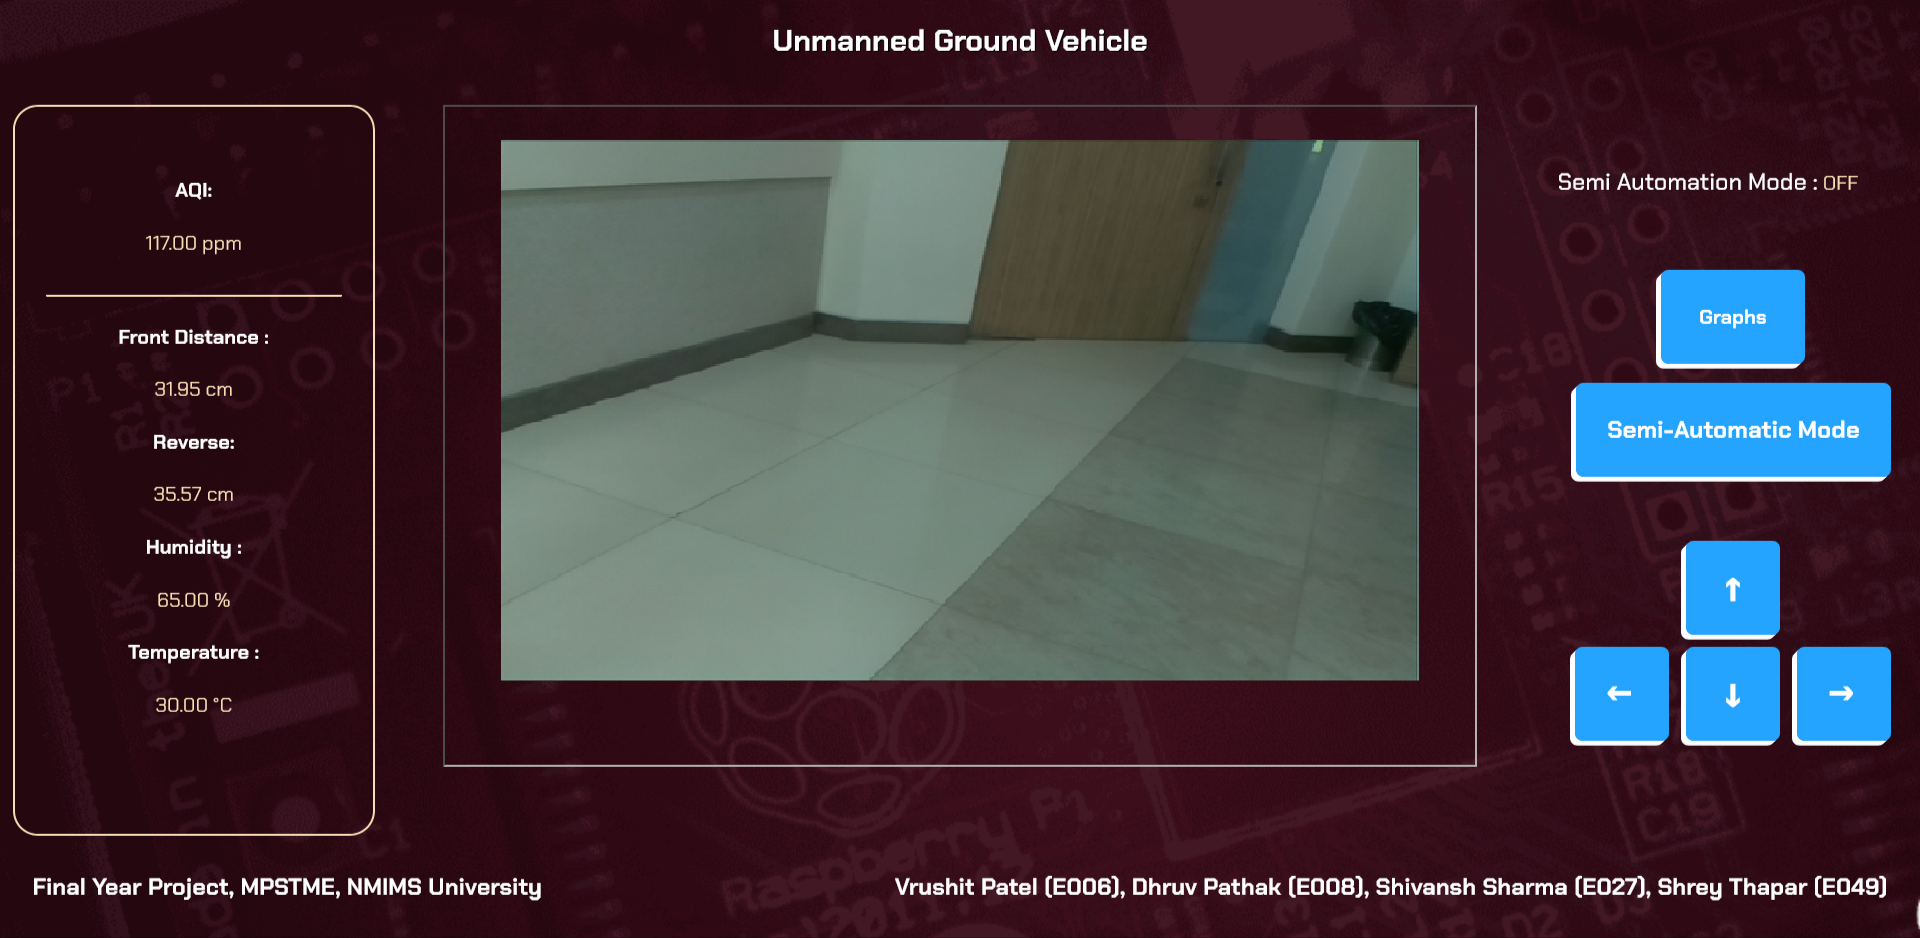
\includegraphics[width=1\linewidth]{website.png}
\caption{Web Application Snapshot}
\label{Fig: Web}
\end{figure*}

\paragraph{Data Module}
The data module displays the data collected from  various sensors on the rover. Data from the sensor is gathered by the Raspberry Pi and sent to a cloud database. The cloud database  sends the data back to the website. Sensors that display data include air quality sensors, ultrasonic sensors, and temperature and humidity sensors. The air quality sensor captures the current air quality around you, and the ultrasonic sensor displays the distance between the  objects closest to the rover. Temperature and humidity sensors are used to detect local humidity and temperature.
\paragraph{Display Module}
The display module helps users navigate the rover  by displaying live feeds from the Pi camera attached to the rover. The live feed is captured by Pi camera and  sent to the Raspberry Pi. Raspberry Pi renders it into an HTML page. Live streams are displayed in this module with an i-frame tag that embeds a local HTML page in the Pi module responsible for the live feed. This live stream is only  possible if the system is connected to a Pi module on your local network.

\paragraph{Utility Module}
The utility module has two buttons. One is for displaying charts and the other is for enabling or disabling the semi-automatic mode of the rover. The data collected by the 
sensors on the rover is visualized and displayed in chart format. The distance between the nearest objects to the rover is plotted as a function of time in the first plot. The second graph plots the data generated by the gyroscope to show the state of the road and shows the z-axis movement over time. The third graph shows the air quality of the area over time. 

One can click the semi-automation button to enter semi-automatic mode. In this mode, the data collected by the ultrasonic sensor in front of the rover can be used by the rover to navigate in the immediate vicinity. The Raspberry Pi processes the data from the sensor and then guides the rover forward to avoid obstacles along the way.

\paragraph{Navigation Module}
The navigation module consists of four buttons. One is for driving forward, the second is for driving to the right, the third is for driving to the left, and the fourth is for driving backward. These buttons allow the user to navigate  around the rover. On clicking the forward button, the Arduino commands all  four DC motors to rotate in the forward direction. The reverse button works as well, with all  four wheels rotating in the reverse direction. The button on the left rotates the motor on the right side of the rover forward when the motor on the left side is stationary. When the user clicks the right button, the motor on the left side of the rover rotates forward and the motor on the right side comes to rest.

\subsection{Architecture}
The rover consists of two processing systems: a Raspberry Pi single board computer and an Arduino UNO micro-controller board. The Raspberry Pi serves as the eye of the system because it consists of a Pi camera that broadcasts live stream around the rover for users to navigate. The Arduino acts as the body of the system because it controls the movement of the four motors that rotate the wheels of the rover. Sensors located on the rover are connected to both the Arduino and Raspberry Pi. The air quality sensor is connected to the Arduino and the temperature and humidity sensor, gyroscope, and  ultrasonic sensors are connected to the Raspberry Pi. To achieve remote access and control of the rover over the Internet, we needed to connect to a cloud database. Therefore, the Raspberry Pi is connected to the Google Firebase cloud server. When the user clicks a navigation button in the web app to move the rover  in a specific direction, the command is sent to Google Firebase, taken from the Raspberry Pi, sent to Arduino using serial communication, and the motor moves accordingly.


\subsection{Data Flow}
As shown in Figure 11, when the user clicks the forward button in the web application to move the rover forward, the forward variable is set to 1. Updating the value of the forward variable does the same thing in the cloud database in real time. The transfer command is then read by the Raspberry Pi on the rover and immediately sends the serialized command  to the Arduino micro-controller  responsible for controlling the motors on the four wheels of the rover. Upon receiving the serialized command, the Arduino will execute the forward code on the hobby motor and the required motor on the rover.

\begin{figure}[ht]
\centering
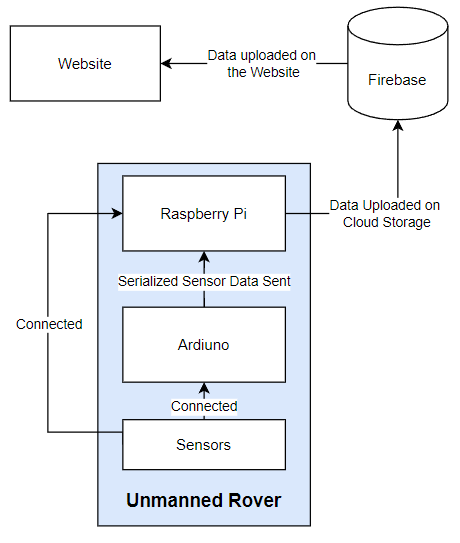
\includegraphics[width=1\linewidth]{sensor.png}
\caption{Sensor Data Flow}
\label{Fig: Data Flow}
\end{figure}

Figure 12 shows another important data flow for the project wherein the data generated by the sensor is consistently displayed in the web application. Some sensors connect to the Arduino micro-controller and others connect to the Raspberry Pi. The data  generated by the sensor connected to the Arduino is first sent  to the Raspberry Pi in serialized format. Once all the sensor data is stored on the Raspberry Pi, the data will be uploaded to Google Firebase's cloud storage and then the data will be successfully transferred to your website.

\section{Limitations}
\begin{enumerate}
        \item When connected to a local WiFi network, the rover responds fairly instantly. The response time increases dramatically when utilising the Internet to operate the rover through a cloud server with a public IP address.
        \item Acquisition of video for live streaming content can only be done on local networks. Live streaming is not possible over WiFi network.
        \item The viewing perspective of the Pi Camera is fixed. This may be overcome by placing the Pi Camera on a high and rotating platform constructed with the assistance of a servo motor.
        \item The processing capabilities of the Raspberry Pi limit the module to points where it cannot perform high-load tasks such as detecting various objects and implementing image processing algorithms. To successfully handle such heavy algorithms, the Raspberry Pi module must support virtual machines or individual processors.
        \item Small objects on the ground or objects at specific angles cannot be detected by the rover's ultrasonic sensors because blind spots are formed as part of an array of the ultrasonic sensors.
\end{enumerate}

\section{Result}
This project provides a comprehensive all-round solution for  rover with the ability to navigate semi-automatically in all directions around. The rover can also be remotely controlled by the user while viewing the live video feed around it using the Pi Camera on the local network. Rover uses a variety of other sensors to display air quality, temperature and humidity, and uses a gyroscope to assess terrain quality. The total cost of manufacturing a rover is about 100 USD, which is significantly lower than the rover models currently retailed. By implementing the adjustments outlined above, our product may be supplied as a comprehensive equipment ideal for industry and domestic surveillance.

\begin{figure}[ht]
\centering
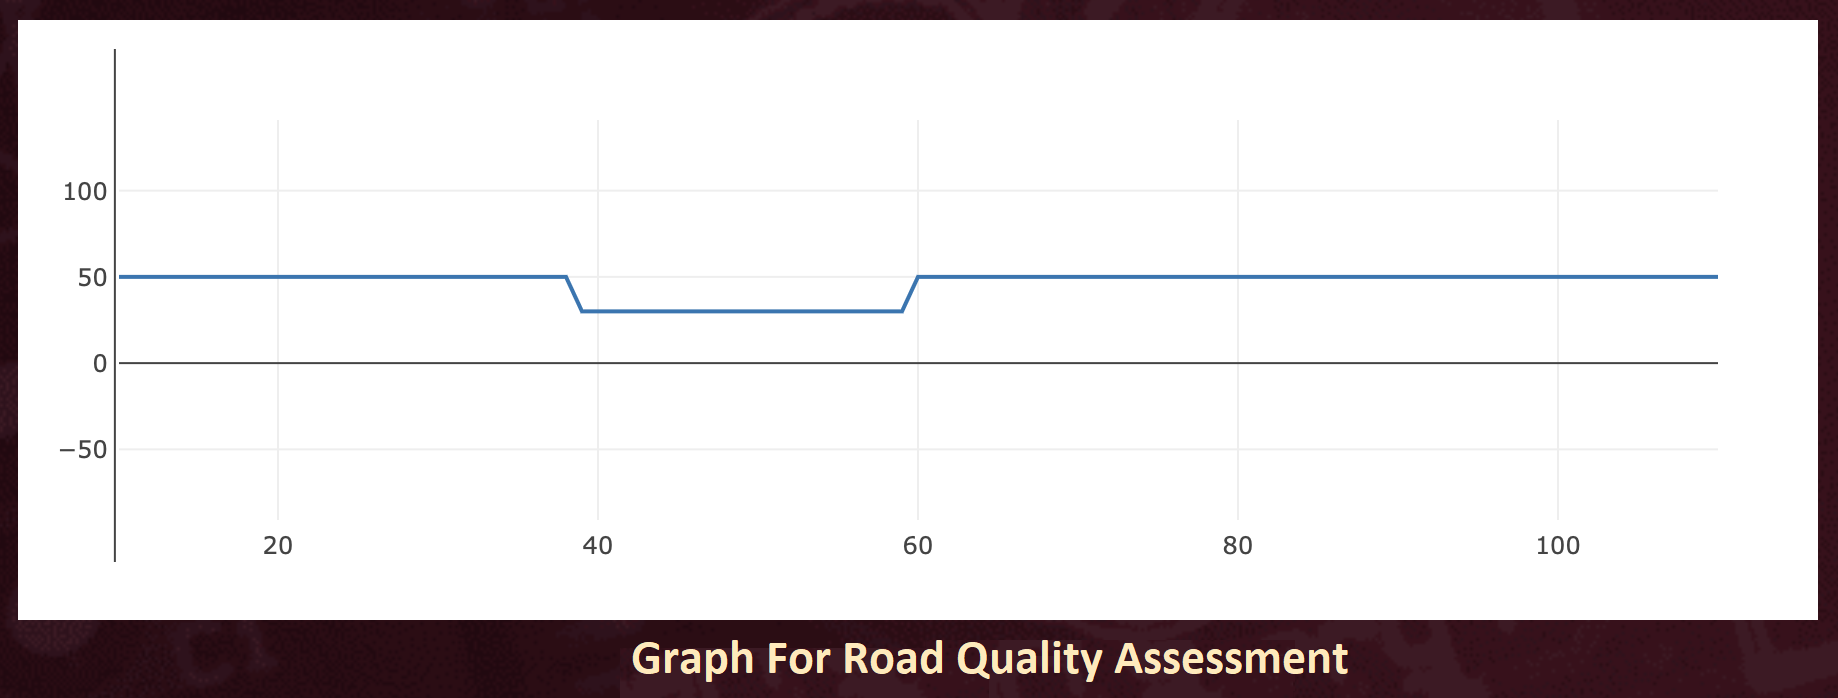
\includegraphics[width=1\linewidth]{Shivi_Send.png}
\caption{Road Quality Graph}
\label{Fig: Road Quality}
\end{figure}

\begin{figure}[ht]
\centering
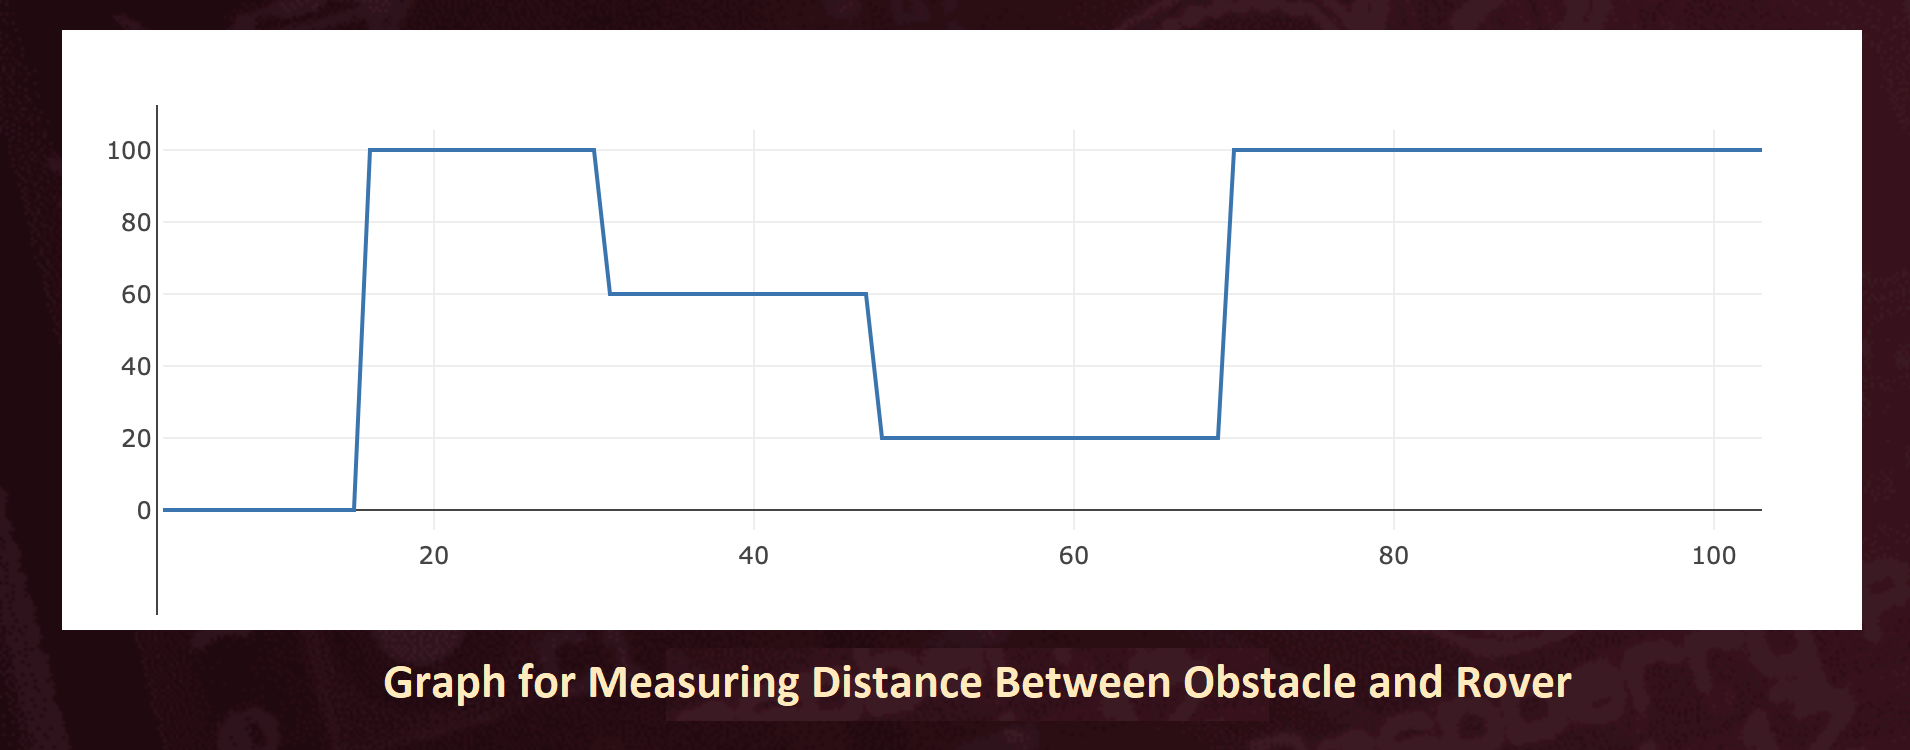
\includegraphics[width=1\linewidth]{Shivi_Send2.png}
\caption{Obstacle Detection}
\label{Fig: Detection}
\end{figure}

\section{Conclusion}

To conclude, the authors would like to state that the unmanned rover gave a balanced perspective on the concept of having a multi-purpose device that could be used for remotely tracking its surroundings, checking the quality of the surface it moves on, and reporting the humidity and temperature of the region. The rover also depended extensively on cloud services for simple activities like movement and web application capability. 
The rover relied on Raspberry Pi and Arduino for practically all of its functions, including sensor interaction, movement, and live broadcast.

\section{Future Scope}
\begin{enumerate}
    \item The rover could be upgraded to withstand uneven surfaces and tolerate different sorts of weather.
    \item By installing solar panels and using compatible batteries to keep the rover independent of battery power and charging issues and to be self-sufficient, the rover's energy efficiency can be significantly increased.
    \item Currently, the rover makes use of Ultrasonic sensors for navigating purposes, however with-inside the future, LiDAR sensors might permit the gadget to create a three-dimensional version of its environment and consequently turning into extra correct in its course and accordingly giving a holistic enjoy to the user.
    \item Pi cameras can be used for object avoidance by implementing an artificial intelligence (machine learning) object avoidance algorithm to automate the movement of the rover. This benefits the rover by avoiding obstacles and dangerous environments and alerting the operator or central station of the danger.
    \item The rover relies on its inbuilt WiFi module for communicating with the cloud server. This could be taken a step ahead by integrating a Long-Term Evolution (LTE) module within the system which would serve the rover to navigate in a wide range of locations.
\end{enumerate}

\begin{thebibliography}{}

\bibitem{8}
Krasniqi X, Hajrizi E
\textit {"Use of IoT technology to drive the automotive industry from connected to full autonomous vehicles"} IFAC-PapersOnLine. 2016 Jan 1;49(29):269-74.

\bibitem{9}
Shirolkar R, Dhongade A, Datar R, Behere G
\textit{" Self-Driving Autonomous Car using Raspberry Pi"}
International Journal of Engineering Research Technology (IJERT) Volume. 2019;8.

\bibitem{3}
H. Mokrani, R. Lounas, M. T. Bennai, D. E. Salhi and R. Djerbi
\textit{"Air Quality Monitoring Using IoT: A Survey,"} 
2019 IEEE International Conference on Smart Internet of Things (SmartIoT), 2019, pp. 127-134.


\bibitem{11}
Ahmed, Syed Hassan and Bouk, Safdar and Kim, Dongkyun and Rawat, Danda B and Song, Houbing
\textit{"Named Data Networking for Software Defined Vehicular Networks."}
2017 IEEE Communications Magazine. 55. 10.1109/MCOM.2017.1601137. 

\bibitem{7}
Tutunji TA, Salah-Eddin M, Abdalqader H
\textit {"Unmanned Ground Vehicle Control using IoT"} In2020 21st International Conference on Research and Education in Mechatronics (REM) 2020 Dec 9 (pp. 1-5). IEEE.

\bibitem{1}
Djama A, Djamaa B, Senouci MR
\textit{"Tcp/ip and icn networking technologies for the internet of things: a comparative study,"}
In 2019 International Conference on Networking and Advanced Systems (ICNAS) 2019 Jun 26 (pp. 1-6). IEEE.

\bibitem{2}
R. Leizerovych, G. Kondratenko, I. Sidenko and Y. Kondratenko
\textit{"IoT-complex for Monitoring and Analysis of Motor Highway Condition Using Artificial Neural Networks,"}
2020 IEEE 11th International Conference on Dependable Systems, Services and Technologies (DESSERT), 2020, pp. 207-212.

\bibitem{5}
Mahmood, Sarmad. (2018)
\textit{"GSM Interaction Based Real Time Climate Change Monitoring Technique,"}
Kirkuk University Journal-Scientific Studies

\bibitem{10}
Bento, Antonio
\textit{IoT: NodeMCU 12e X Arduino Uno, Results of an experimental and comparative survey} 
2018. 6. 45-56. 

\bibitem{4}
Kamalakannan M, Devadharshini K. 
\textit{"Controlling the Speed of Conveyor Belt using Python – Raspberry Pi 3B+,"}
Orient.J. Comp. Sci. and Technol;12(2).

\bibitem{12}
N. A. Mathew and K. M. Abubeker
\textit{"IoT based real time patient monitoring and analysis using Raspberry Pi 3,"} 
2017 International Conference on Energy, Communication, Data Analytics and Soft Computing (ICECDS), 2017, pp. 2638-2640

\bibitem{20}
Szymon Wojtyła, Piotr Klama and Tomasz Baran 
\textit{Is 3D printing safe? Analysis of the thermal treatment of thermoplastics: ABS, PLA, PET, and nylon} 2017 Journal of Occupational and Environmental Hygiene

\bibitem{13}
Manon Kok, Jeroen D. Hol and Thomas B. Sch 
\textit{”Using Inertial Sensors for Position and Orientation Estimation”} Foundations and Trends in Signal Processing: Vol. 11: No. 1-2, pp 1-153. 

\bibitem{14}
Kanade, Prakash and Alva, Prajna.
\textit{RASPBERRY PI PROJECT -ULTRASONIC DISTANCE SENSOR IN CIVIL ENGINEERING} 
2020. International Journal in IT and Engineering (IJITE) Volume 8 Issue 10, October

\bibitem{15}
Qiongzheng Lin, Zhenlin An, and Lei Yang. 
\textit{Rebooting Ultrasonic Positioning Systems for Ultrasound-incapable Smart Devices.} 
2019. The 25th Annual International Conference on Mobile Computing and Networking Article 2, 1–16.

\bibitem{16}
Bryan J. Hubbell, Amanda Kaufman, Louie Rivers, Kayla Schulte, Gayle Hagler, Jane Clougherty, Wayne Cascio, Dan Costa
\textit{Understanding social and behavioral drivers and impacts of air quality sensor use}
2018 Science of The Total Environment

\bibitem{19}
K. Chang, P. Rammos, S. A. Wilkerson, M. Bundy, S. Andrew Gadsden, 
\textit{"LiPo battery energy studies for improved flight performance of unmanned aerial systems,"} 
2016 Unmanned Systems Technology XVIII, 98370W

\bibitem{18}
H. Suryoatmojo
\textit{"Design Li-Po Battery Charger with Buck Converter under Partially CC-CV Method,"}
2020 International Seminar on Intelligent Technology and Its Applications (ISITIA)

\bibitem{6}
N. Hossain, M. T. Kabir, T. R. Rahman, M. S. Hossen and F. Salauddin
\textit{"A real-time surveillance mini-rover based on OpenCV-Python-JAVA using Raspberry Pi 2,"} 
2015 IEEE International Conference on Control System, Computing and Engineering (ICCSCE), 2015, pp. 476-481.

\bibitem{17}
R. Petija, M. Glevaňák, M. Kucan, P. Fecil'ak and F. Jakab
\textit{"Experimental Implementation of TinyIPFIX Protocol for Arduino and Raspberry Pi Platform,"} 
2020 18th International Conference on Emerging eLearning Technologies and Applications (ICETA)


\end{thebibliography}
\end{document}